\problem5
Read Daan Frenkel's
``Why colloidal systems can
be described by statistical mechanics:
some not very original comments on
the Gibbs paradox'' ({\sl Mol. Phys.},
112:2325--2329, 2014).
We have posted this article on Canvas, under `Homework'.
Summarize the primary conclusion in one sentence or less.
\solution{\\
Entropy is a quantity we {\bf define} to characterize 
the collective behavior of particles, 
and contains a constant factor shift
determined by our ability to distinguish between
these particles macroscopically.
(The shift depends on the `resolution'
we view our system at, i.e. how precisely
we can differentiate between different species.
This `resolution' is really the level
of detail we {\bf choose} to study for our system---quantum 
mechanical indistinguishability is, in a sense,
an upper limit on this resolution). 
}

\bigskip
\problem{15}
The partition function describing rotational degrees of freedom
in ideal diatomic molecules is given by:
\begin{equation}
q_\text{rot} = 
\sum_{l=0}^\infty (2l+1) \exp\left[-\frac{\hbar^2}{2\mu R^2 \kB T}l(l+1)\right] 
\label{eq:qrot}
\end{equation}
In class, we replaced the summation with an integral over $l$
and found that $q_\text{rot} \simeq T/\theta_\text{rot}$,
where $\theta_\text{rot} \equiv \frac{\hbar^2}{2\mu R^2 \kB}$.

\smallskip\subp
We can improve the integral approximation by using
the Euler-Maclaurin summation formula:
\[ \sum_{n=a}^{b} f(n) = \int_a^b f(n)\, \dd n
 + \frac{f(a) + f(b)}{2}
 - \frac{f^{(1)}(a) - f^{(1)}(b)}{12}
 + \frac{f^{(3)}(a) - f^{(3)}(b)}{720}
 + \cdots \]
$f^{(1)}$ and $f^{(3)}$ denote first and third derivatives.
Apply this formula to Eq.~(\ref{eq:qrot}), and show that
\[ q_\text{rot} =
  \frac{T}{\theta_\text{rot}} + \frac{1}{3} + \frac{1}{15} \frac{\theta_\text{rot}}{T}
+ \mathcal{O}\left(\frac{\theta_\text{rot}^2}{T^2}\right) \]
\solution{
Using the definition of $\theta_{\rm rot}$, define $I$ and $u(l)$ such that:
\[ I \equiv \int_0^\infty \dd l \, (2l+1) 
            \exp \left[-\frac{\theta_{\rm rot}}{T} l (l+1) \right] 
     \equiv \int_0^\infty \dd l \, u(l) \]
Using the Euler-Maclaurin summation formula (up to third order), 
$q_{\rm rot}$ can be written as:
\[ q_{\rm rot} = I + \frac{u(0) + u(\infty)}{2}
               - \frac{u^{(1)}(0) - u^{(1)}(0)}{12} 
               + \frac{u^{(3)}(0) - u^{(3)}(\infty)}{720}
               + \ldots \]
We need the first three derivatives of $u(l)$. 
Looking at the problem statement, drop 
higher powers of $\theta_{\rm rot}/T$ 
since we know that $\theta_{\rm rot} \ll T$
for rotational modes at room temperature.
\begin{align*}
         u(l) &= (2l+1) \exp \left[ -\frac{\theta_{\rm rot}}{T}l(l+1) \right] \\
   u^{(1)}(l) &= \left( 2 - \frac{\theta_{\rm rot}}{T} (2l + 1)^2  \right)
                 \exp \left[ -\frac{\theta_{\rm rot}}{T}l(l+1)     \right] \\
   u^{(2)}(l) &= \left(  -6   \frac{\theta_{\rm rot}}{T} (2l+1)    \right)
                 \exp \left[ -\frac{\theta_{\rm rot}}{T}l(l+1)     \right] 
               + \mathcal{O} \left( \frac{\theta_{\rm rot}^2}{T^2} \right) \\
   u^{(3)}(l) &= \left( -12   \frac{\theta_{\rm rot}}{T}           \right)
                 \exp \left[ -\frac{\theta_{\rm rot}}{T}l(l+1)     \right] 
               + \mathcal{O} \left( \frac{\theta_{\rm rot}^2}{T^2} \right) 
\end{align*}
Now, evaluate the summation formula:
\begin{align*}
  q_{\rm rot} &= I + \frac{u(0) + u(\infty)}{2}
               - \frac{u^{(1)}(0) - u^{(1)}(\infty)}{12} 
               + \frac{u^{(3)}(0) - u^{(3)}(\infty)}{720} \\
              &= \frac{T}{\theta_{\rm rot}}
               + \frac{1 + 0}{2}
               - \frac{(2 - \theta_{\rm rot}/T) - 0}{12} 
               + \frac{(-12\,\theta_{\rm rot}/T) - 0}{720} 
               + \mathcal{O} \left( \frac{\theta_{\rm rot}^2}{T^2} \right) \\
             &= \frac{T}{\theta_{\rm rot}}
              + \left( \frac{1}{2} - \frac{1}{6} \right)
              + \frac{\theta_{\rm rot}}{T}
                \left( \frac{1}{12} - \frac{1}{60} \right)
              + \mathcal{O} \left( \frac{\theta_{\rm rot}^2}{T^2} \right) \\
             &= \frac{T}{\theta_{\rm rot}} + \frac{1}{3}
              + \frac{1}{15} \left( \frac{\theta_{\rm rot}}{T} \right) 
              + \mathcal{O} \left( \frac{\theta_{\rm rot}^2}{T^2} \right)
\end{align*}
This is exactly what we wanted to show:
\[ \boxed{ q_{\rm rot} 
        = \frac{T}{\theta_{\rm rot}} + \frac{1}{3}
        + \frac{1}{15} \left( \frac{\theta_{\rm rot}}{T} \right) 
        + \mathcal{O} \left( \frac{\theta_{\rm rot}^2}{T^2} \right) } \]
}

\smallskip\subp
Use your result from (a) to calculate the error 
incurred by using $q_{\rm rot} \simeq T/\theta_{\rm rot}$ 
for (1) $\rm N_2$\,(g) at 300\,K;
and (2) $\rm H_2$\,(g) at 300\,K.
The reduced mass is given by
$\mu = m_1 m_2 / (m_1 + m_2)$,
and the inter-atomic distance $R$ is 
$1.094$\,\AA\ for $\rm N_2$ and
$0.742$\,\AA\ for $\rm H_2$.
\solution{\\
Denote the summation-corrected result $q_{\rm sum}$
and the integral-only approximation $q_{\rm int}$:
\[ e = \frac{|q_{\rm sum} - q_{\rm int}|}{q_{\rm sum}} \]
(i) For $N_2$ gas at $300$ K (mind your units):
\begin{align*}
  \mu_{N_2} &= 1.16*10^{-26}\,{\rm kg} \\
  \theta_{\rm rot,N_2} &= 2.90\,{\rm K} \\
  e_{N_2} &= 0.0032 = 0.32\,\%
\end{align*}
(ii) For $H_2$ gas at $300$ K:
\begin{align*}
  \mu_{H_2} &= 8.30*10^{-28}\,{\rm kg} \\
  \theta_{\rm rot,H_2} &= 88.4\,{\rm K} \\
  e_{H_2} &= 0.094 = 9.4\,\%
\end{align*}
\[ \boxed{ \text{Error in N}_2:~0.32\,\% \quad , \quad
           \text{Error in H}_2:~9.4\,\% } \]
Qualitatively, this makes sense.
The error caused by using an integral approximation 
is larger for $H_2$ than $N_2$ because
$H_2$ has a larger rotational temperature,
which is close to the same order of magnitude
as room temperature.
}


\smallskip\subp
The calculations above demonstrate that,
at normal conditions,
all the rotational modes of a diatomic ideal gas have been excited.
Thus, the temperature dependence of heat capacity should 
arise primarily from vibrational modes. 
Experimentally measured heat capacities for CO\,(g) 
at different temperatures are tabulated below.
\[ \begin{array}{rc}
   T/{\rm K} & C_V/(N \kB) \\
   \hline
     300 & 2.455 \\
     400 & 2.538 \\
     500 & 2.621 \\
     600 & 2.689 \\
     700 & 2.764 \\
     800 & 2.833 \\
     900 & 2.928 \\
    1000 & 2.992 \\
    1100 & 3.019 \\
    1200 & 3.107 \\
    1300 & 3.154 \\
    1400 & 3.221 \\
    1500 & 3.243 \\
\end{array} \]
%$$ \frac{C_\text{V}}{N\kB} = 2.192 + (9.240\times10^{-4}{\rm K^{-1}})T 
%- (1.41\times10^{-7}{\rm K^{-2}})T^2 $$
%Plot $C_\text{V}/(N\kB)$ versus $T$ over this range,
Estimate $\theta_\text{vib}$ for CO\,(g) 
by fitting this data to the result we derived in class:
\[ \frac{C_\text{V}}{N\kB} = \frac{5}{2} +
\left(\frac{\theta_\text{vib}}{T}\right)^2 \frac{\ee^{-\theta_\text{vib}/T}}
{(1 - \ee^{-\theta_\text{vib}/T})^2} . \]
Report your fitted value for $\theta_\text{vib}$ and 
plot the tabulated data and your best fit on the same graph.
({\sl Note: The actual vibrational temperature for {\rm CO} 
      is $\theta_\text{vib} = 3107\,$K.})
\solution{\\
Using \texttt{NonlinearModelFit[]} in Mathematica:
\[ \boxed{ \theta_{\rm vib} \approx 2,990\,{\rm K} } \] \\
\begin{center}
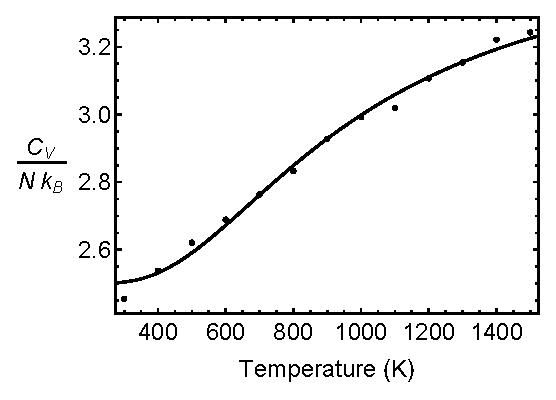
\includegraphics[width=0.6\textwidth,height=!]{hw5plot}
\end{center}
\newpage
}


\bigskip
\problem{40}
Computing the partition function
for interacting (non-ideal) molecules is generally difficult.
However, in low-density gases with only short-ranged interactions,
a virial expansion can be used 
to estimate thermodynamic potentials.
Consider a box of $N$ identical gas molecules.
The configuration of this system can be uniquely specified by
the positions  $\{\rv_i\} = \{\rv_1, \rv_2, \ldots, \rv_N\}$
and momenta $\{\vv p_i\} = \{\vv p_1, \vv p_2, \ldots, \vv p_N\} $
of all the molecules.
The energy of each configuration
can be written, generally,
as the sum of kinetic $K$ and potential energy $U$:
\begin{align*}
E &= K(\{\vv p_i\}) + U(\{\rv_i\}) \\
  &= \sum_{i=1}^{N} \frac{\vv p_i^2}{2 m} +  \Biggl(\,
     \underbrace{\sum_{i=1}^N \sum_{j=i+1}^N u^{(2)}(\rv_i, \rv_j)}_\text{2-body potential} +
     \underbrace{\sum_{i=1}^N \sum_{j=i+1}^N \sum_{k=j+1}^N
     u^{(3)}(\rv_i, \rv_j, \rv_k)}_\text{3-body potential}
     + \cdots \Biggr)
\end{align*}
Above, $m$ is the mass per molecule.
The potential energy has been decomposed
into a sum of 2-body interactions, 3-body interactions, etc.
The terms $u^{(2)}$ and $u^{(3)}$ are placeholders
for the functional forms of the inter-molecular interactions,
and will depend explicitly on the positions $\{\rv_i\}$.

\smallskip \subp
Using the grand canonical ensemble $(\mu, V, T)$,
show that the pressure $p$ of this system is:
\def\intr{\int\!\dd\rv}
% KH - I moved the def to get rid of a weird leading indentation
\[ p = \frac{\kB T}{V} \ln\left(
   1 + \sum_{N=1}^\infty \frac{\lambda^N}{N!} Z_N \right). \]
Here $\lambda \equiv \frac{e^{\beta\mu}}{\Lambda^3}$ is
proportional to the fugacity,
$\Lambda$ is the thermal de~Broglie wavelength we defined in class,
and $Z_N$ is the reduced configurational partition function given by:
\[ Z_N = Z_N(V,T) \equiv
  \intr_1\intr_2\cdots\intr_N\, e^{-\beta U(\rv_1, \rv_2, \ldots, \rv_N)} . \]
\solution{\\
Remember that the grand canonical partition function
is related to the potential $pV$:
\[ p = \frac{\kT}{V} \ln \Xi
     = \frac{\kT}{V} \ln
       \left[ \sum_i \exp \left( \frac{-E_i + \mu N_i}{\kT} \right) \right] \]
It is convenient to convert the summation into integrals.
The summation is unitless, so we must 
normalize (non-dimensionalize) the integral representation.
\[\sum_i = \sum_{N=0}^\infty \sum_{\rv_i}^\infty 
           \sum_{{\vv p}_j}^\infty 
         = \sum_{N=0}^\infty \left[
           \left( \prod_{i=1}^N \frac{1}{V}
                  \int \dd \rv_i \right)
           \left( \prod_{j=1}^N \frac{V}{h^3}
                  \int \dd {\vv p}_j \right) \right] \]
In the above, $h$ is Planck's constant,
and we  use $1/N!$ to 
account for indistinguishability. 
\begin{align*}
 p &= \frac{\kT}{V} \ln \left[ \sum_i \exp \left( 
                        \frac{-E_i + \mu N_i}{\kT} \right) \right] \\
   &= \frac{\kT}{V} \ln \left[ 
      \sum_{N = 0}^\infty \frac{e^{-\beta \mu N_i}}{N!}
      \left( \prod_{i=1}^N \frac{1}{V}
             \int \dd \rv_i \, e^{-\beta U\{\rv_i\}} \right)
      \left( \prod_{j=1}^N \frac{V}{h^3}
             \int \dd {\vv p}_j \, e^{-\beta K\{ {\vv p}_j \}} \right) \right] 
\end{align*}
Remember that $\{\rv_i\} = \{\rv_1,\rv_2,\ldots,\rv_N\}$
and $\{ {\vv p}_j \} = \{ {\vv p}_1, {\vv p}_2, \ldots, {\vv p}_N \}$.
The first term in parentheses
is related to the partition function $Z_N$
defined in the problem statement.
\[ \prod_{i=1}^N \frac{1}{V} \int \dd \rv_i \, e^{-\beta U\{\rv_i\}} 
 = \frac{Z_N}{V^N} \]
The second integral relates to the ideal gas
partition function we evaluated in class.
\[ \prod_{j=1}^N \frac{V}{h^3} 
   \int \dd {\vv p}_j \, e^{-\beta K\{ {\vv p}_j \}}
 = \left( \frac{(2 \pi m \kT)^{3/2}}{h^3} \right)^N 
 = V^N \left( \frac{1}{\Lambda^3} \right)^N \]
Simplification is now straightforward:
\begin{align*}
 p &= \frac{\kT}{V} \ln \left[ \sum_{N=0}^\infty 
      \frac{e^{\beta \mu N}}{N!}
      \left( \frac{Z_N}{V^N} \right)
      \left( \frac{V^N}{\Lambda^{3N}} \right) \right] \\
   &= \frac{\kT}{V} \ln \left[ \sum_{N=0}^\infty \frac{Z_N}{N!} 
      \left( \frac{e^{\beta \mu}}{\Lambda^3} \right)^N
      \right] 
    = \frac{\kT}{V} \ln \left[ 
      \frac{Z_0}{1} (1) +
      \sum_{N=1}^\infty \frac{Z_N}{N!}
      \left( \lambda \right)^N \right] \\
   &= \frac{\kT}{V} \ln \left[ 1 + 
      \sum_{N=1}^{\infty} \frac{ Z_N \lambda^N}{N!} \right]
\end{align*}
Thus, we have shown that:
\[ \boxed{ p = \frac{\kT}{V} \ln \left( 1 + \sum_{N=1}^\infty 
               \frac{\lambda^N}{N!} Z_N \right) } \]
}

\smallskip \subp
The virial expansion is particularly useful for low-density fluids.
Since the chemical potential of a classical ideal gas is given by
$\mu = \kB T \ln(\rho \Lambda^3)$,
the parameter $\lambda$ is of the same order as density, $\rho$.
This allows us to write a Taylor expansion for the pressure:
\begin{equation}
p = \kT \sum_{n=1}^{\infty} b_n \lambda^n .
\label{eq:pvirial}
\end{equation}
Show that the first three coefficients are given by:
\begin{align*}
b_1 = \frac{Z_1}{V},\quad
b_2 = \frac{1}{2\,V}\left(Z_2 - Z_1^2\right),\quad
b_3 = \frac{1}{6\,V}\left(Z_3 - 3Z_1 Z_2 + 2Z_1^3\right).
\end{align*}
This clearly shows that the coefficients $b_n$
are functions of $V$ and $T$, i.e., $b_n = b_n(V,T)$.
\solution{\\
We need to Taylor expand the solution from (a)
to third order (three coefficients).
First, define $s$ to be the summation from part (a):
\[ s \equiv \sum_{N=1}^\infty \frac{\lambda^N}{N!} Z_N 
          = \lambda Z_1 + \frac{\lambda^2}{2} Z_2 
          + \frac{\lambda^3}{6} Z_3 + \ldots \]
In a low-density fluid, we are given that $\lambda \simeq \rho$,
such that $\lambda \ll 1$. We assume, quite reasonably,
that in this case $s \ll 1$. Taylor expand the log term from (a):
\[ \ln (1 + s) \approx s - \frac{s^2}{2} + \frac{s^3}{3} + \ldots \]
Substitute in $s$, truncating to third order in $\lambda$
(i.e. drop higher order terms):
\begin{align*}
\ln (1 + s) &\approx \left( \lambda Z_1 + \frac{\lambda^2}{2} Z_2 
                            + \frac{\lambda^3}{6} Z_3 \right)  
                  - \frac{1}{2} \left( \lambda^2 Z_1^2 
                          + \frac{2 \lambda^3}{2} Z_1 Z_2 \right) 
                  + \frac{1}{3} \left( \lambda^3 Z_1^3 \right) \\
           &= \lambda   \left( Z_1 \right) 
            + \lambda^2 \left( \frac{Z_2}{2} - \frac{Z_1^2}{2} \right)
            + \lambda^3 \left( \frac{Z_3}{6} - \frac{Z_1 Z_2}{2} 
                             + \frac{Z_1^3}{3} \right)
\end{align*}
We can now rewrite the solution from (a) as:
\[ \boxed{ p \approx \kT 
           \left[ \lambda   \left( \frac{Z_1}{V} \right) 
                + \lambda^2 \left( \frac{Z_2 - Z_1^2}{2 V} \right) 
                + \lambda^3 \left( \frac{Z_3 - 3 Z_1 Z-2 + 2 Z_1^3}
                                               {6V} \right) \right] } \]
By matching powers of $\lambda$, clearly:
\[ \boxed{ b_1 = \frac{Z_1}{V} \quad , \quad 
           b_2 = \frac{Z_2 - Z_1^2}{2V} \quad , \quad 
           b_3 = \frac{Z_3 - 3 Z_1 Z_2 + 2 Z_1^3}{6V} } \]
}

\smallskip \subp
Write down an expression for the average number of molecules 
$\ave{N}$,
then use Eq.~(\ref{eq:pvirial}),
the Taylor expansion for pressure,
to show that density $\rho = \frac{\ave{N}}{V}$ is given by
\begin{equation}
\rho = \sum_{n=1}^\infty n\, b_n \lambda^n .
\label{eq:rholambda}
\end{equation}
\solution{
\[ \boxed{ \ave{N} = \kT \pdc{\ln \Xi}{\mu}{V,T} 
                   = \pdc{(\kT \ln \Xi)}{\mu}{V,T} 
                   = \pdc{(pV)}{\mu}{V,T} } \]
\begin{align*}
  \ave{N} &= \pd{}{\mu} \left[ \kT V \sum_{n=1}^\infty 
                               b_n (V,T) \lambda^n \right]_{V,T} 
           = \kT V \pd{}{\lambda} 
             \left[ \sum_{n=1}^\infty 
                    b_n (V,T) \lambda^n \right]_{V,T} 
             \pdc{\lambda}{\mu}{V,T} \\
          &= \kT V \left[ \sum_{n=1}^\infty n\,b_n \lambda^{n-1} \right]
             \left( \frac{\lambda}{\kT} \right) 
           = V \sum_{n=1}^\infty n\,b_n \lambda^n
\end{align*}
Naturally, simply divide $\ave{N}$ by $V$ to get density.
\[ \boxed{ \rho \equiv \frac{\ave{N}}{V}
 = \sum_{n=1}^\infty n\,b_n \lambda^n } \]
}

\smallskip \subp
In order to convert the Taylor series for pressure
into a series over density, 
we must invert Eq.~(\ref{eq:rholambda}).
One way to achieve this is to introduce
$\lambda = \sum_{n=1}^{\infty} a_n \rho ^n$.
Substitute $\lambda$ into Eq.~(\ref{eq:rholambda})
by matching coefficients,
and then show that the lower-order coefficients are related by:
\[ a_1 = b_1^{-1} = 1,\quad
   a_2 = -2\, b_2,\quad
   a_3 = 8\,b_2^2 - 3\, b_3. \]
{\bf Hint}: $Z_1 = V$ is needed to show $b_1 = 1$.
\solution{ \\
Let's quickly check the hint. Assume there is no 1-body potential,
such that $U(\rv_1) = 0$. 
This is equivalent to assuming homogeneous density,
as we don't care about constant shifts in energy. 
\[ Z_1 = \int \dd \rv_1 \, e^{-\beta U(\rv_1)} = \int \dd \rv_1 = V \]
From part (b), $b_1 = Z_1/V = V/V = 1$, as desired. 
Truncate to third-order terms:
\begin{align*}
  \rho &= b_1 \lambda + 2 b_2 \lambda^2 + 3 b_3 \lambda^3 + \ldots \\
       &=   b_1 \left( a_1 \rho + a_2 \rho^2 + a_3 \rho^3 + \ldots \right) 
        + 2 b_2 \left( a_1 \rho + a_2 \rho^2 + a_3 \rho^3 + \ldots \right)^2
        + 3 b_3 \left( a_1 \rho + a_2 \rho^2 + a_3 \rho^3 + \ldots \right)^3 \\              
       &=   b_1 \left( a_1 \rho + a_2 \rho^2 + a_3 \rho^3 + \ldots \right) 
        + 2 b_2 \left( a_1^2 \rho^2 + 2 a_1 a_2 \rho^3 + \ldots \right)
        + 3 b_3 \left( a_1^3 \rho^3 + \ldots \right) \\
       &= (a_1 b_1) \rho + (a_2 b_1 + 2 a_1^2 b_2) \rho^2 
        + (a_3 b_1 + 4 a_1 a_2 b_2 + 3 a_1^3 b_3) \rho^3 + \mathcal{O}(\rho^4)
\end{align*}
In order to enforce equality, the leading coefficient must be one, 
and all other coefficients (on powers of $\rho$) must be zero.
\begin{align*}
   &a_1 b_1 = a_1 (1) = 1 \\
   &\Rightarrow ~ a_1 = b_1^{-1} = 1 \\ \\
   &a_2 b_1 + 2 a_1^2 b_2 = a_2 (1) + 2 (1)^2 b_2 = a_2 + 2 b_2 = 0 \\
   &\Rightarrow ~ a_2 = -2 b_2 \\ \\
   &a_3 b_1 + 4 a_1 a_2 b_2 + 3 a_1^3 b_3 
  = a_3 (1) + 4 (1) (-2 b_2) b_2 + 3 (1)^3 b_3 
  = a_3 - 8 b_2^2 + 3 b_3 = 0 \\
  &\Rightarrow ~  a_3 = 8 b_2^2 - 3 b_3
\end{align*}
Therefore, by matching coefficients, we have shown that:
\[ \boxed{ a_1 = b_1^{-1} = 1 \quad,\quad 
           a_2 = -2 b_2 \quad,\quad 
           a_3 = 8 b_2^2 - 3 b_3} \]
}

\smallskip \subp
Now substitute the $\lambda$ series into
Eq.~(\ref{eq:pvirial}),
the Taylor expansion for pressure, and show that
\[ p = \rho \kT \left[ 1 - b_2 \rho +
       \left(4\, b_2^2 - 2\, b_3\right) \rho^2 + \ldots \right]. \]
This result indicates that
the second and third order virial coefficients are:
\[ B_2 = - b_2,\quad B_3 = 4\,b_2^2 - 2\,b_3. \]
\solution{ 
\[ p = \kT \sum_{n=1}^\infty b_n \lambda^n
     = \kT \left[ b_1 \lambda + b_2 \lambda^2 + b_3 \lambda^3 + \ldots \right] \]
Again, keeping only terms to cubic order in $\rho$:
\begin{align*}
  \frac{p}{\kT}
    &= b_1 \left( a_1 \rho + a_2 \rho^2 + a_3 \rho^3 + \ldots \right) 
     + b_2 \left( a_1 \rho + a_2 \rho^2 + a_3 \rho^3 + \ldots \right)^2
     + b_3 \left( a_1 \rho + a_2 \rho^2 + a_3 \rho^3 + \ldots \right)^3 \\              
  &=   b_1 \left( a_1 \rho + a_2 \rho^2 + a_3 \rho^3 + \ldots \right) 
     + b_2 \left( a_1^2 \rho^2 + 2 a_1 a_2 \rho^3 + \ldots \right)
     + b_3 \left( a_1^3 \rho^3 + \ldots \right) \\
  &= (a_1 b_1) \rho + (a_2 b_1 + a_1^2 b_2) \rho^2 
   + (a_3 b_1 + 2 a_1 a_2 b_2 + a_1^3 b_3) \rho^3 + \mathcal{O}(\rho^4) \\
  &\approx (1) \rho + (-2b_2(1) + (1)^2 b_2) \rho^2 
   + ((8b_2^2 - 3b_3)(1) + 2(1)(-2b_2)(b_2) + (1)^3 b_3)) \rho^3 \\
  &= \rho \left[ 1 - b_2 \rho + (4 b_2^2 - 2 b_3) \rho^2 \right]
\end{align*}
Therefore, we have shown that:
\[ \boxed{ p = \rho \kT \left[ 1 - b_2 \rho 
             + (4 b_2^2 - 2 b_3) \rho^2 + \ldots \right] }\]
}

\smallskip \subp
Remarkably, the second order virial coefficient 
{\it only} depends on the 2-body interaction.
The 2-body potential $u^{(2)}(\rv_i, \rv_j)$ frequently
depends only on the inter-molecular separation $|\rv_i - \rv_j|$, i.e.,
$u^{(2)}(\rv_i, \rv_j) = u(|\rv_i - \rv_j|)$.
Using this fact, and $b_2 = \frac{1}{2V}(Z_2 - Z_1^2)$ from part (b),
show that:
\[ B_2 %= \frac{1}{2} \intr \left(1 - e^{-\beta u(|\rv|)}\right)
 = 2\pi \int_0^\infty\!\dd r\, r^2 \left(1 - e^{-\beta u(r)} \right)  . \]
This expression enables 
estimation of 2-body interaction parameters
from measurements of the second virial coefficient.
Similar expressions can be derived
for the third, and all other higher-order virial coefficients.
\solution{
\[ B_2 = -b_2 = \frac{1}{2V} (Z_1^2 - Z_2) \]
We showed in part (d) that $Z_1 = V$.
Now, evaluate $Z_2$:
\[ Z_2 = \int \dd \rv_1 \int \dd \rv_2 \, e^{-\beta U(\rv_1, \rv_2) } 
       = \int \dd \rv_1 \int \dd \rv_2 \, e^{-\beta u(|\rv_1-\rv_2|) } \]
Having a functional dependence on $|\rv_1-\rv_2|$ effectively
reduces the double integral into a single integral,
plus a volume factor.
The easiest way to think about this is that
the integral is invariant with respect
to simultaneous translation of $\rv_1$ and $\rv_2$. 
We can simply fix $\rv_2 = 0$ and be done with it.
Simplify the integral:
\[ Z_2 = \int \dd \rv_1 \int \dd \rv_2 \, e^{-\beta u(|\rv_1-\rv_2|) } 
       = V \int \dd \rv \, e^{-\beta u(|\rv|) } \]
Convert to spherical coordinates, as $u = u(|\rv|)$
(only magnitude of $r$ matters):
\begin{align*}
  Z_2 &= V \int \dd \rv \, e^{-\beta u(|\rv|) }
       = V \int_0^\pi \dd \phi \int_0^{2\pi} \dd \theta 
           \int_0^\infty \dd r \, e^{-\beta u(r)} r^2 \sin(\phi) \\
      &= 4 \pi V \int_0^\infty \dd r \, r^2 e^{-\beta u(r)}
\end{align*}
We're really close!
\begin{align*}
B_2 &= \frac{1}{2V} \left[ V^2 - 4 \pi V 
       \int_0^\infty \dd r \, r^2 e^{-\beta u(r)} \right]
     = \frac{1}{2} \left[ V - 4 \pi 
       \int_0^\infty \dd r \, r^2 e^{-\beta u(r)} \right] \\
    &= \frac{1}{2} \left[ \int_0^\infty \dd r \, (4 \pi r^2) -
       4 \pi \int_0^\infty \dd r \, r^2 e^{-\beta u(r)} \right] \\
    &= 2 \pi \int_0^\infty \dd r \, r^2 \left( 1 - e^{-\beta u(r)} \right)
\end{align*}
Above, we converted $V$ back into an
integral in spherical coordinates.
We're done!
\[ \boxed{ B_2 = 2 \pi \int_0^\infty \dd r \, r^2 
                 \left( 1 - e^{-\beta u(r)} \right) } \]
}

\smallskip \subp
Let's look for the virial expansion of entropy.
For the sake of simplicity, we focus only on
leading order corrections.
Up to second order in the virial expansion, 
the pressure can be written as
$p = \rho \kT (1 + B_2 \rho)$.
Entropy can be obtained from the Gibbs-Duhem relation,
$V \dd p = N \dd \mu + S \dd T$.
Show that it can be written
\begin{equation}
S = N \kB (1 + B_2 \rho) +
N \kT B_2'\rho +
V \kT (1 + 2 B_2 \rho)
\left.\frac{\partial \rho}{\partial T}\right|_{\mu}.
\label{eq:Svirial}
\end{equation}
where $B_2' = \frac{\dd B_2}{\dd T}$
can be evaluated from the explicit expression
derived in part~(3.f).
\solution{\\
Reading directly from the Gibbs-Duhem relation:
\[ \frac{S}{V} = \pdc{p}{T}{\mu} 
 = \pd{}{T} \left[ \rho \kT 
   \left( 1 + B_2 \rho + \ldots \right) \right]_\mu \]
Above, $\rho$ and $B_2$ can have a temperature dependence. 
Apply the product rule liberally:
\begin{align*}
  \frac{S}{V} &=
    \pdc{\rho}{T}{\mu} \kT (1 + B_2 \rho) 
  + \rho \kB (1 + B_2 \rho)
  + \rho \kT \left[ B_2 \pdc{\rho}{T}{\mu} + \rho \pdc{B_2}{T}{\mu} \right] \\
 &= \rho \kB (1 + B_2 \rho) + \rho^2 \kT B'_2 + \kT (1 + 2 B_2 \rho) 
    \left. \pd{\rho}{T} \right|_{\mu}
\end{align*}
Since $\rho = \frac{\ave{N}}{V}$, the thermodynamic $N$
is given by $N = \rho V$. Thus:
\[ \boxed{ S = N \kB (1 + B_2 \rho) + N \kT B'_2 \rho 
             + V \kT (1 + 2 B_2 \rho) \left. \pd{\rho}{T} \right|_{\mu} } \]
}

\smallskip \subp
The remaining unknown,
$\left.\frac{\partial \rho}{\partial T}\right|_{\mu}$,
can be obtained in many ways.
One efficient approach is to use the virial
expansion for $\lambda$ from part~(3.d).
Using the relation between $\lambda$ and chemical potential,
(i) show that, to the linear order in $B_2$,
the chemical potential can be written:
\begin{align*}
\quad \mu = \kT \left[
  \ln\left(\rho \Lambda^3\right) + 2 B_2 \rho \right].
\end{align*}
The first term is ideal gas chemical potential,
and the second is the second virial correction.
Setting $\dd \mu = 0$,
and noting that both $\Lambda$ and $B_2$ depends
on temperature, (ii) show that
$$
\left.\frac{\partial \rho}{\partial T}\right|_{\mu}
= - \frac{\rho}{T} \frac{\ln\left(\rho\Lambda^3\right)
  + 2B_2\rho + 2TB_2'\rho - 3/2} {1 + 2 B_2\rho} .
$$
Substituting the above to Eq.~(\ref{eq:Svirial}),
(iii) show that the entropy is given by
$$
S = N\kB \left[\, 5/2 - \ln\left(\rho\Lambda^3\right)
\right] - N\kB \bigl(B_2 + TB_2'\bigr) \rho .
$$
The first term is the ideal gas entropy we derived in class.
The second term, linear in density,
represents the lowest order
correction due to inter-molecular interactions.
The virial expansion for all other thermodynamic potentials
can be trivially derived from those for $p$, $\mu$, and $S$.
For instance, the expansion for total energy
is given by $U = \mu N + TS - pV$.
Similarly, we could have found an expression for entropy
by first calculating the Helmholtz free energy $F = \mu N - pV$,
and then by applying $S = - (\partial F / \partial T)_{N, V}$.
The result is identical to the expression above.
\solution{\\
(i) Since $\lambda = e^{\beta \mu}/\Lambda^3$,
$\beta \mu = \ln (\lambda \Lambda^3)$.
Substituting in 
$ \lambda = a_1 \rho + a_2 \rho^2 + \ldots
  \approx \rho + 2 B_2 \rho^2$:
\[ \beta \mu \approx \ln \left[ \Lambda^3 (\rho + 2 B_2 \rho^2) \right]
 = \ln \left[ \Lambda^3 \rho (1 + 2 B_2 \rho) \right]
 = \ln(\Lambda^3 \rho) + \ln(1 + 2 B_2 \rho) \]
The virial series expansion is based on $B_2 \rho$ being small 
(the higher order terms must get smaller).
Therefore, we Taylor expand $\ln (1 + 2 B_2 \rho) \approx 2 B_2 \rho + \ldots$ to get:
\[ \boxed{ \mu = \kT \left[ \ln(\rho \Lambda^3) + 2 B_2 \rho \right] } \]
(ii) $\mu = \mu(T,\rho)$:
\[ \dd \mu = \pdc{\mu}{T}{\rho} \dd T + \pdc{\mu}{\rho}{T} \dd \rho \]
If we set $\dd \mu = 0$, clearly:
\[ \pdc{\rho}{T}{\mu} = - \pdc{\mu}{T}{\rho} \pdc{\mu}{\rho}{T}^{-1} \]
Evaluate the partials, noting that
$\frac{\dd \Lambda}{\dd T} = -\frac{\Lambda}{2T}$:
\begin{align*}
\pdc{\mu}{T}{\rho} 
   &= \kB \left[\ln (\rho \Lambda^3) + 2 B_2 \rho \right] 
    + \kT \left[ - \frac{3 \Lambda^2}{\Lambda^3} 
      \left( \frac{\Lambda}{2 T} \right) + 2 \rho B'_2 \right] \\
   &= \kB \left[ \ln(\rho \Lambda^3) + 2 B_2 \rho
    - \frac{3}{2} + 2 \rho T B'_2 \right] \\
\pdc{\mu}{\rho}{T} &= \kT \left[ \frac{1}{\rho} + 2 B_2 \right] 
    = \frac{\kT}{\rho} \left[ 1 + 2 B_2 \rho \right]
\end{align*}
Using these expressions, it is clear that:
\[ \boxed{ \pdc{\rho}{T}{\mu} = - \frac{\rho}{T} 
           \frac{\ln(\rho \Lambda^3) 
               + 2 B_2 \rho + 2T B'_2 \rho - 3/2}
                {1 + 2 B_2 \rho} } \]
(iii) Start by evaluating the term with the partial of $\rho$:
\begin{align*}
     V \kT (1 + 2 B_2 \rho) \left. \pd{\rho}{T} \right|_{\mu} 
  &= - (\rho V) \kB \left[ \ln(\rho \Lambda^3) + 2 B_2 \rho 
                          + 2 T B'_2 \rho - 3/2 \right] \\
  &= -N \kB \ln(\rho \Lambda^3) + \frac{3 N \kB}{2} 
     -2 N \kB B_2 \rho - 2 N \kB T B'_2 \rho
\end{align*}                   
\begin{align*}
  S &= N \kB (1 + B_2 \rho) + N \kT B'_2 \rho 
     + V \kT (1 + 2 B_2 \rho) \left. \pd{\rho}{T} \right|_{\mu} \\
    &= N \kB (1 + 3/2) - N \kB \ln(\rho \Lambda^3) 
     + N \kB B_2 \rho (1 - 2) + N \kT B'_2 \rho (1 - 2) \\
\end{align*}
\[ \boxed{ S = N \kB \left[ 5/2 - \ln(\rho \Lambda^3) \right] 
             - N \kB (B_2 + T B'_2) \rho } \]
}
